\documentclass[report.tex]{subfiles}
\begin{document}

This chapter consists of two parts:
the first part presents the data of the experiments described above as-is,
and the second part discusses the results in the light of the thesis hypotheses.
The aim of this chapter is to verify or discard the hypotheses, and will
conclude with a summary of the thesis results.
This conclusion will be discussed in a broader context in the subsequent chapter.

Details on the system that performed the benchmarks as well as
library versions and experiment code is available in Appendix
\ref{app:experiment}.
\\[0.1cm]

During the experimental phase, name the evaluation of the parallel model on
NEST, an incompatibility of the DSL with the PyNN framework was discovered.
During the initialisation of the weights PyNN threw an exception in the 
merge layer.
The error was due to the fact that a single population receives weights
from multiple populations, which requires a \textit{view} or a subset of the
population. 
In PyNN this is done using indices, and a consistency check is carried out to
verify that the index is within a certain range.
However, the parallel layer requires that the indices are configured out of
order, resulting in a failed index verification check.

While all the models compile and pass the structural tests of PyNN,
the experiments using the Merge layer fail to complete.
As a consequence the parallel spiking experiments are unavailable, and are
marked as N/A in the result tables below.
A complete description of the error trace is available in Section
\ref{lst:pynn_exception} on page \pageref{lst:pynn_exception}.

The metric used to compare the performance of the results is the prediction
accuracy of the models. 
The one-hot outputs are compared to the labels, and given $N$ experiments and
$K$ true hits, the accuracy is defined as $K / N$.
Thus, an accuracy of 1 is a perfect score, and 0 indicates that none of the
labels have been correctly predicted.

\section{NAND}
Both the NAND and XOR experiments are built by compiling the expression 
\texttt{\textbf{dense} 2 4 $\obar$ \textbf{dense} 4 2}.
The input data is generated by randomly sampling two numbers between 0 and 1.
The resulting NAND value was then used as the target label.
The networks were injected with a total of 512 data points, corresponding to 8
batches.

Data from the NAND experiments are shown in Table \ref{tab:nand}.
Futhark achieves a 100\% accuracy rate as expected.
However, the rates are below chance level (0.75 for NAND) in NEST, both during
the random weight initialisation and while transferring weights from Futhark.
It is noteworthy that the accuracy increases significantly when the Futhark weights are
injected.

Standard deviations for NEST are small in the case of random weights, meaning
that the variance between the experiment accuracies are small.
This variance becomes significantly larger when the weights are transferred into NEST from
Futhark.
This could be explained by the fact that the optimised model in Futhark does not
correlate with an equal 'plateau' in NEST. 
In turn this indicates that the gradient model for NEST is different, although
not necessarily worse.
The NEST prediction rate, however, proves that the gradient model is incomplete at
best.

\def\arraystretch{1.2}
\begin{table}
  \begin{tabular}{r|l l}
  Backend & Random weights & Transferred weights \\ \hline
  Futhark & 1.000 & - \\
  NEST & 0.370 $\pm$ 0.040 & 0.69 $\pm$ 0.216\\ 
  \end{tabular}
  \caption{Mean accuracies and standard deviations of the NAND experiment.}
  \label{tab:nand}
\end{table}

Figure \ref{fig:nand_snn_error} shows a plot of the average backpropagated errors of
the model.
The gradient errors are interesting to explore because the relative values reveal
the average performance of the model (smaller is better), and the absolute
values describe how well the model is able to cancel out errors entirely.
The plot shows that the errors never approaches zero, but are instead hovering
around 45.

In the present experiment the errors decrease initially, but begin to increase
after the third batch.
The model with imported weights shows a higher accuracy in the beginning, 
but rapidly decreases to the same level as the model with randomly initialised
weights.
The declining error rates show that the model is capable of learning to a
certain degree.
The later reversal means that the optima for the gradient models does not align
with the spiking model.
This can either be caused by an initially effective, but erroneous 
gradient model, or an imprecise translation scheme from the raw input data to
input currents.

\begin{figure}
  \includegraphics[width=\linewidth]{images/nand.png}
  \caption{Mean gradient error rates for the NAND network simulated in NEST. The rates
  are produced by averaged over 10 simulations.}
  \label{fig:nand_snn_error}
\end{figure}
\FloatBarrier

\section{XOR}
Tabel \ref{tab:xor} shows the results of the XOR experiment.
The experiment execution and generation of data is similar to the NAND
experiment above, except from the label generation that was based on the NAND
logical gate.

The chance level of the XOR experiment is at 0.5, lower than for the NAND
experiment.
Futhark reaches the same accuracy rate of 100\%.
Notably, NEST performs above chance level, but only with a small margin. The 
weight improvements when transferring the Futhark parameters are smaller than 
what was seen in the NAND experiment.

\begin{table}
  \begin{tabular}{r l l}
  Backend & Random weights & Transferred weights \\ \hline
  Futhark & 1.000 & - \\ 
  NEST & 0.530 $\pm$ 0.038 & 0.585 $\pm$ 0.033 \\
  \end{tabular}
  \caption{Mean accuracies and standard deviations of the XOR experiment.}
  \label{tab:xor}
\end{table}

Figure \ref{fig:xor_snn} illustrates the summed error rates for the XOR
experiment, and a similar behaviour as in the NAND experiment can be observed:
the error decreases initially, but increases again after the third batch has
been processed.
The experiment shows a similar learning behaviour as above, although with a
higher accuracy.
In combination with the imprecise gradient models, this is likely due to the
nature of the XOR task.
In the case of the NAND task, only 25\% of the data trains the second 'on' bit
in the one-hot vector. 
With a constant learning rate, this means that the model is not allowed to move
sufficiently in the direction of the gradient, before another data points pulls
the model in another direction. 
For the XOR task this is different because 50\% of the data trains the second on
bit.

The gradient error rates for the XOR network plotted in Figure \ref{fig:xor_snn} shows
same picture as with the NAND error rates: they decline initially, but grows
after the third batch has been processed.

\begin{figure}
  \includegraphics[width=\linewidth]{images/xor.png}
  \caption{Mean gradient error rates for the XOR network simulated in NEST. The rates
  are produced by averaged over 10 simulations.}
  \label{fig:xor_snn}
\end{figure}

\FloatBarrier

\section{Sequential MNIST}
Table \ref{tab:mnist_seq} and Table \ref{tab:mnist_par} display the mean
accuracies of the sequential and parallel MNIST experiments respectively.
The state-of-the-art models for MNIST has achieved an accuracy rate of 99.88\%
\cite{LeCun2019}.
As a comparison, the chance level for MNIST is 0.1 because there are 10 possible output labels.

While the Futhark models was tested on the full
70000 images of the MNIST data, the data for the NEST experiments were reduced to 
8192 data points (128 batches) to avoid excessive runtimes.
Despite this reduction in size the NEST experiments took
well over 6 hours to complete.

Futhark performs equally well in the two experiments with a mean accuracy of
0.710. 
However, this result is still far below contemporary results.
The state-of-the-art models are to a large part based on convolutions instead of
non-linear activations, although some models achieve similarly high accuracies
with only densely connected layers.

The current experiments are challenged by a) the data compression, b) a constant
learning rate and a model that is too small to accurately capture the complexity
of the problem domain.

The sequential results on NEST performs close to chance level with randomly
initialised weights perform close to chance level.
The standard deviation is quite small, indicating that the results are
consistent across runs.
However, the 0.047\% is negligible and proves that the gradient model
and input translations are incorrect.

It is noteworthy that the model with the transferred rates performs worse than
the randomly initialised weights.
This is unexpected and questions the assumption that the weights are correctly
transferred between the \gls{ANN} and \gls{SNN} models, especially because the
standard deviations are so small that it cannot be ascribed to chance.

\begin{table}
  \begin{tabular}{r l l}
  Backend & Random weights & Transferred weights \\ \hline
  Futhark & 0.710 & - \\ 
  NEST & 0.147 $\pm$ 0.044 & 0.098 $\pm$ 0.006 \\
  \end{tabular}
  \caption{Mean accuracies and standard deviations for the sequential MNIST experiment.}
  \label{tab:mnist_seq}
\end{table}

\begin{table}
  \begin{tabular}{r l l}
  Backend & Random weights & Transferred weights \\ \hline
  Futhark & 0.710 & - \\ 
  NEST & N/A & N/A \\
  \end{tabular}
  \caption{Mean accuracies and standard deviations for the parallel MNIST experiment.}
  \label{tab:mnist_par}
\end{table}

\begin{figure}
  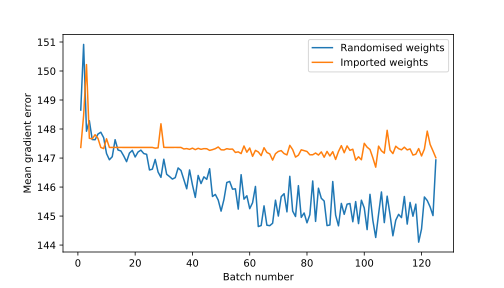
\includegraphics[width=\linewidth]{images/mnist_snn.png}
  \caption{Summed gradient error rates for the sequential MNIST network simulated in NEST. The rates
  are produced following each batch and are averaged over 10 simulations.}
  \label{fig:mnist_snn}
\end{figure}
\FloatBarrier

Figure \ref{fig:mnist_snn} shows the summed gradient error rates for the MNIST
models.
Unlike the above experiments the rates does not improve initially.
Instead they worsen shortly in the beginning, again indicating that they are not training towards
the correct gradients.
The constant high gradient error values aligns with this interpretation by
stagnating and thus failing to find better minima.

There is a clear difference between the model with randomised weights and with
non-randomised weights.
It is counterintuitive that the errors in the model with the imported parameters
performs the worst.
If this was consistent with the NAND and XOR experiments, the accuracies would
be better initially, but trail off after the advantage of the
imported weights disappears.
One possible explanation is that the imported weight model found a consistent
local minima that it could not escape from.
It is even feasible that the minima is global in the linear non-spiking gradient
model, but that the coding scheme fails to translate the minima into the correct
weights.
\\[0.1cm]

Looking at the data from the experiments in depth, a large number of 
`dead neurons' can be found.\index{dead neuron}
`Dead neurons` are neurons whose weights have decreased to a point where they are not able to
fire anymore.
This is detrimental to the result because of the argmax classification that
brings the network closer to chance level.
Because the gradients are calculated based on the ReLU model, such a low neuron
activity level is difficult to compensate for, since the activations approaches
0, where the ReLU model is non-differentiable.\index{ReLU}
\\[0.1cm]

The low mean accuracies when performing the NEST experiments suggest that the approximated
gradient spiking model is flawed.
The visualisations show that the initial models are capable of performing some form of
learning, but that the learning is imprecise and quickly looses
momentum.
This can be attributed to a large number of causes, but in the light of the
consistently high backpropagation error rates, this is likely due to the
aforementioned flawed gradient model and too many dead neurons.

However, the error rates in the weight transfer models are smaller than, or
close to, those in the random weight initialisation models.
The weak improvements does not decisively prove that there is a relation between
the models in Futhark and the models in NEST, but it does not disprove it.

Regarding learning, the spiking models are showing signs of 
improvements, albeit inconsistent signs. 
Both the NAND and the XOR experiments are achieving a consistently lower error
rate.
The randomised MNIST model shows the same consistent development, but this
development is difficult to reason about in the light of the weight transfer
model, where the error gradient roughly remains constant.
\end{document}
